\HeaderQuote{But it's no use going back to yesterday, because I was a different person then.}{Alice}

\chapter{Peer-reviewed conference papers}\label{app:confpapers} \todo[color=green!40]{\cref{app:confpapers} Unfinished}

\section[LION5]{Supervised Learning Linear Priority Dispatch Rules for Job-Shop Scheduling}\label{app:lion5}
Supervised Learning Linear Priority Dispatch Rules for Job-Shop Scheduling was submitted by \citeauthor{InRu11a} to \emph{Learning and Intelligent OptimizatioN Conference} (LION 5), January 17-21, 2011, Rome, Italy. The paper was been accepted as long paper (original novel and unpublished work) for presentation at the conference and inclusion in the proceedings. 

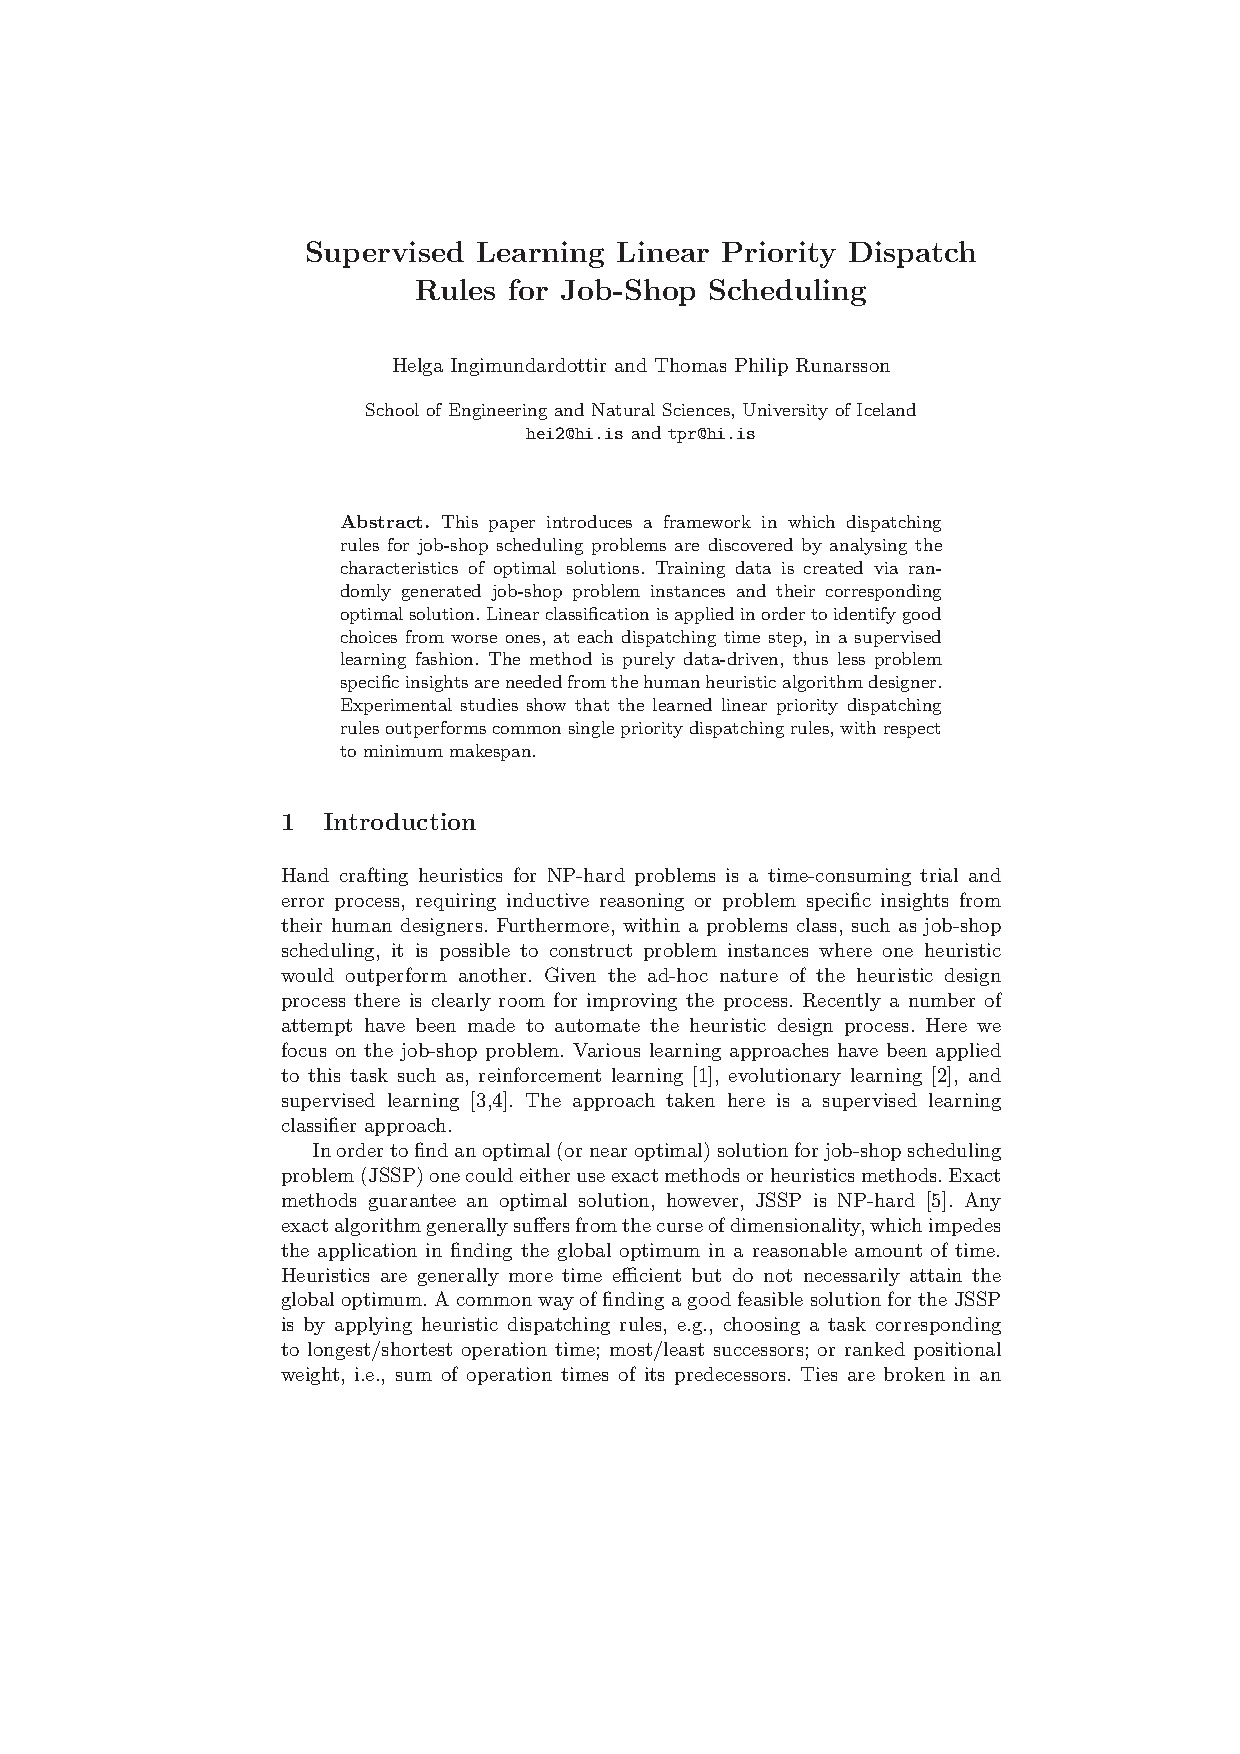
\includepdf[pages=1-15,pagecommand={\thispagestyle{fancy}}]{papers/lion5_linearJSP.pdf}

\section[ISDA11]{Sampling Strategies in Ordinal Regression for Surrogate Assisted Evolutionary Optimization}\label{app:isda2011}
Sampling Strategies in Ordinal Regression for Surrogate Assisted Evolutionary Optimization was submitted by \citeauthor{InRu11b} to \emph{11th International Conference on Intelligent Systems Design and Applications} (ISDA 11), November 22-24, 2011, Córdoba, Spain. The paper was accepted for presentation at the conference and for publication in the conference proceedings published by IEEE.

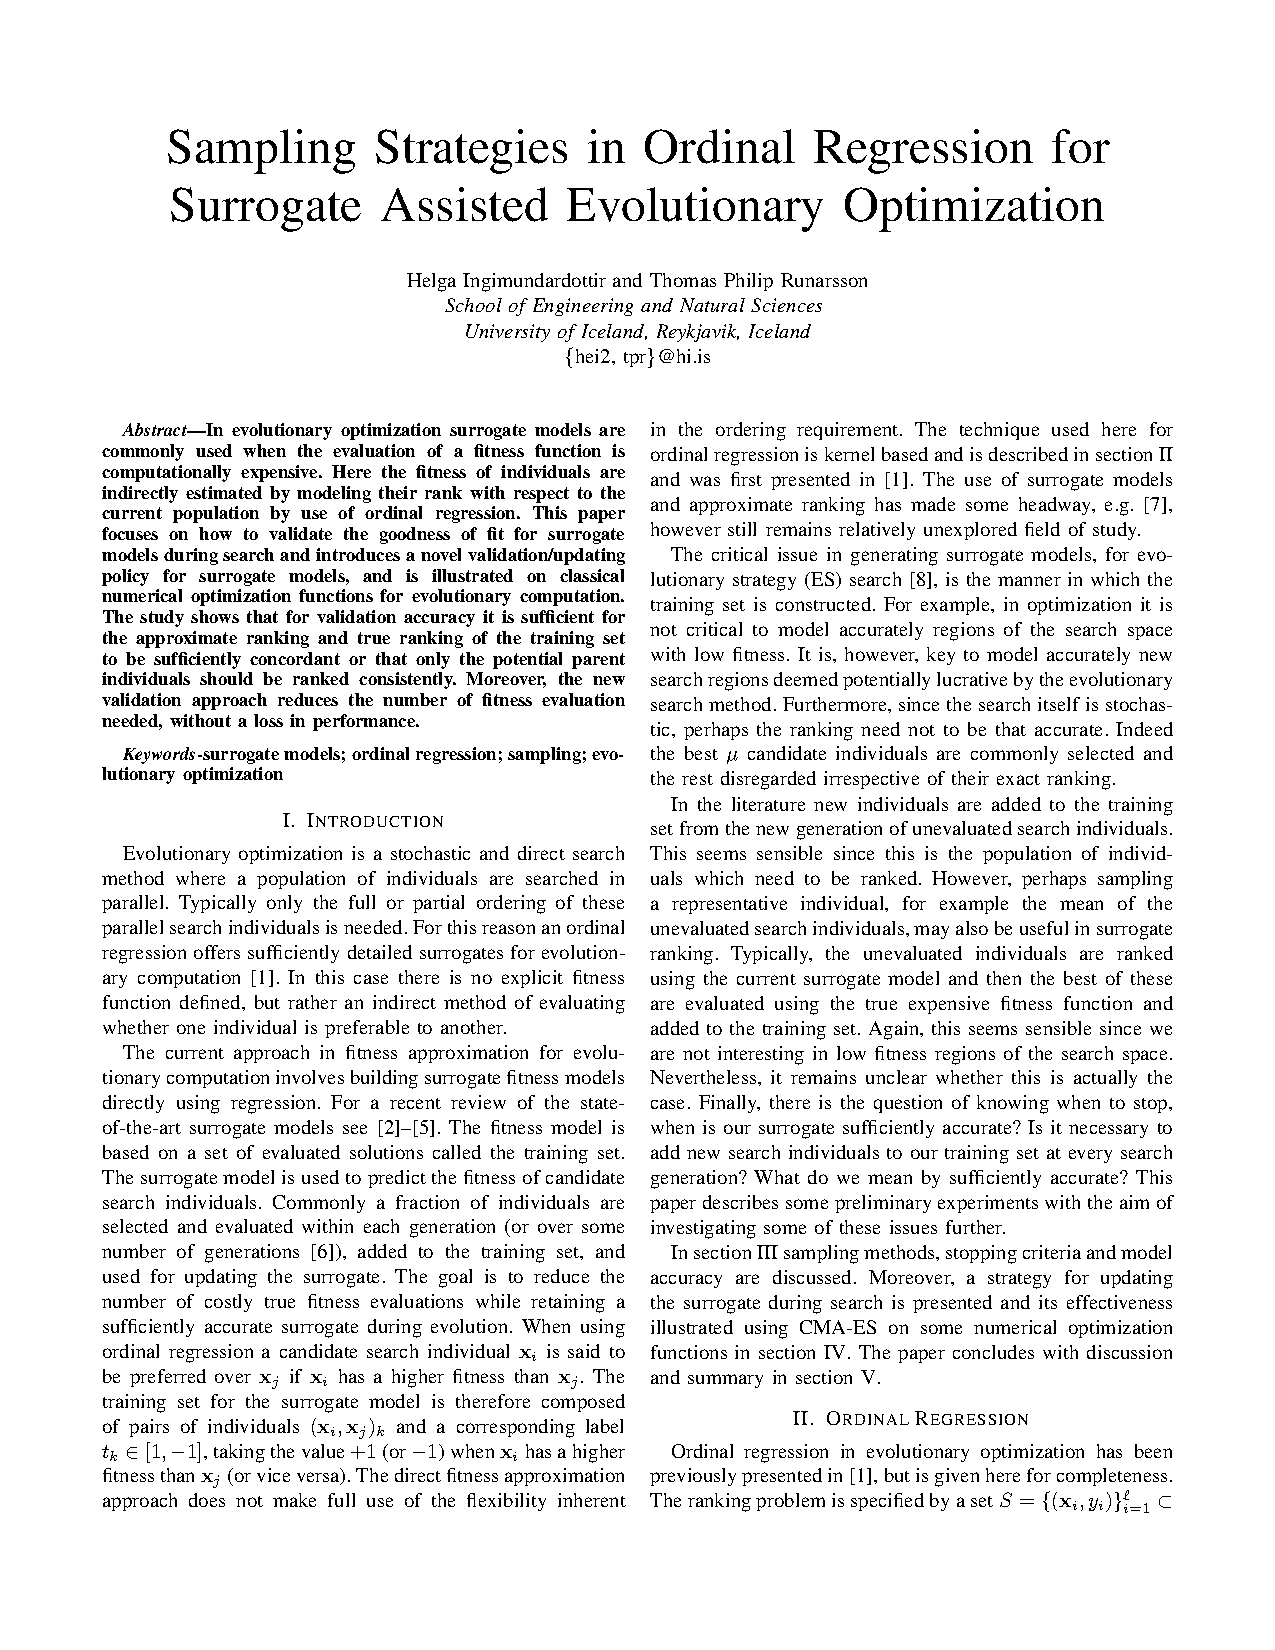
\includepdf[pages=1-6,pagecommand={\thispagestyle{fancy}}]{papers/isda2011.pdf}% ath. ekki blaðsíðutal með á IEEE double-column formattinu. Mögulega hægt ef það væri hægt að scale-a síðurnar betur niður. 

\section[LION6]{Determining the Characteristic of Difficult Job Shop Scheduling Instances for a Heuristic Solution Method}\label{app:lion6}
Determining the Characteristic of Difficult Job Shop Scheduling Instances for a Heuristic Solution Method was submitted by \citeauthor{InRu12} to \emph{Learning and Intelligent OptimizatioN Conference} (LION 6), January 16-20, 2012, Paris France. The paper was been accepted as short paper (an extended abstract of novel work) for presentation at the conference and inclusion in the proceedings. 

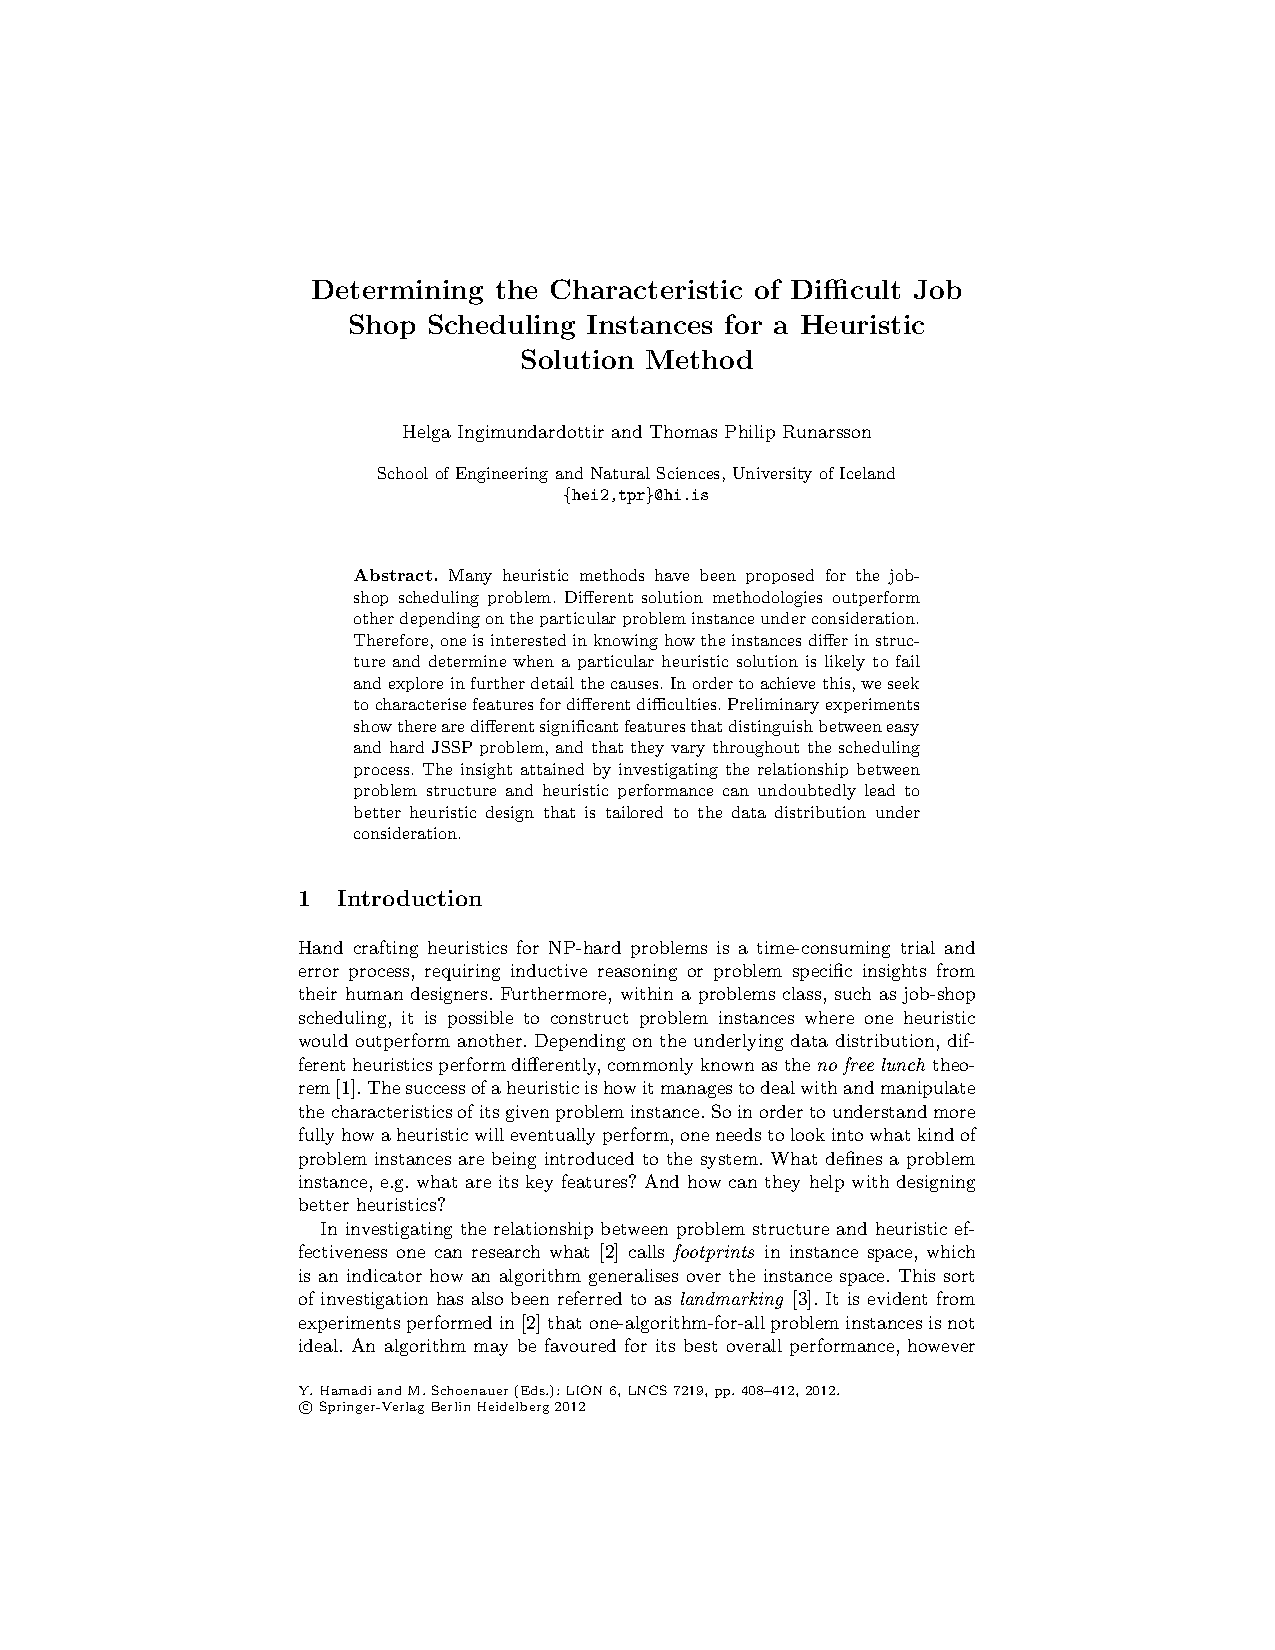
\includepdf[pages=1-5,pagecommand={\thispagestyle{fancy}}]{papers/lion6_easyhardJSSP.pdf}

\section[GECCO14]{Evolutionary Learning of Weighted Linear Composite Dispatching Rules for Scheduling}\label{app:gecco14}
Evolutionary Learning of Weighted Linear Composite Dispatching Rules for Scheduling was submitted by \citeauthor{InRu14a} to \emph{Genetic and Evolutionary Computation Conference} (GECCO 14), July 12-16, 2014, Vancouver, Canada. %The paper was been accepted as long paper (original novel and unpublished work) for presentation at the conference and inclusion in the proceedings. 

\todo[inline]{Find out how to include GECCO pdf. includepdf doesn't work as it should.}

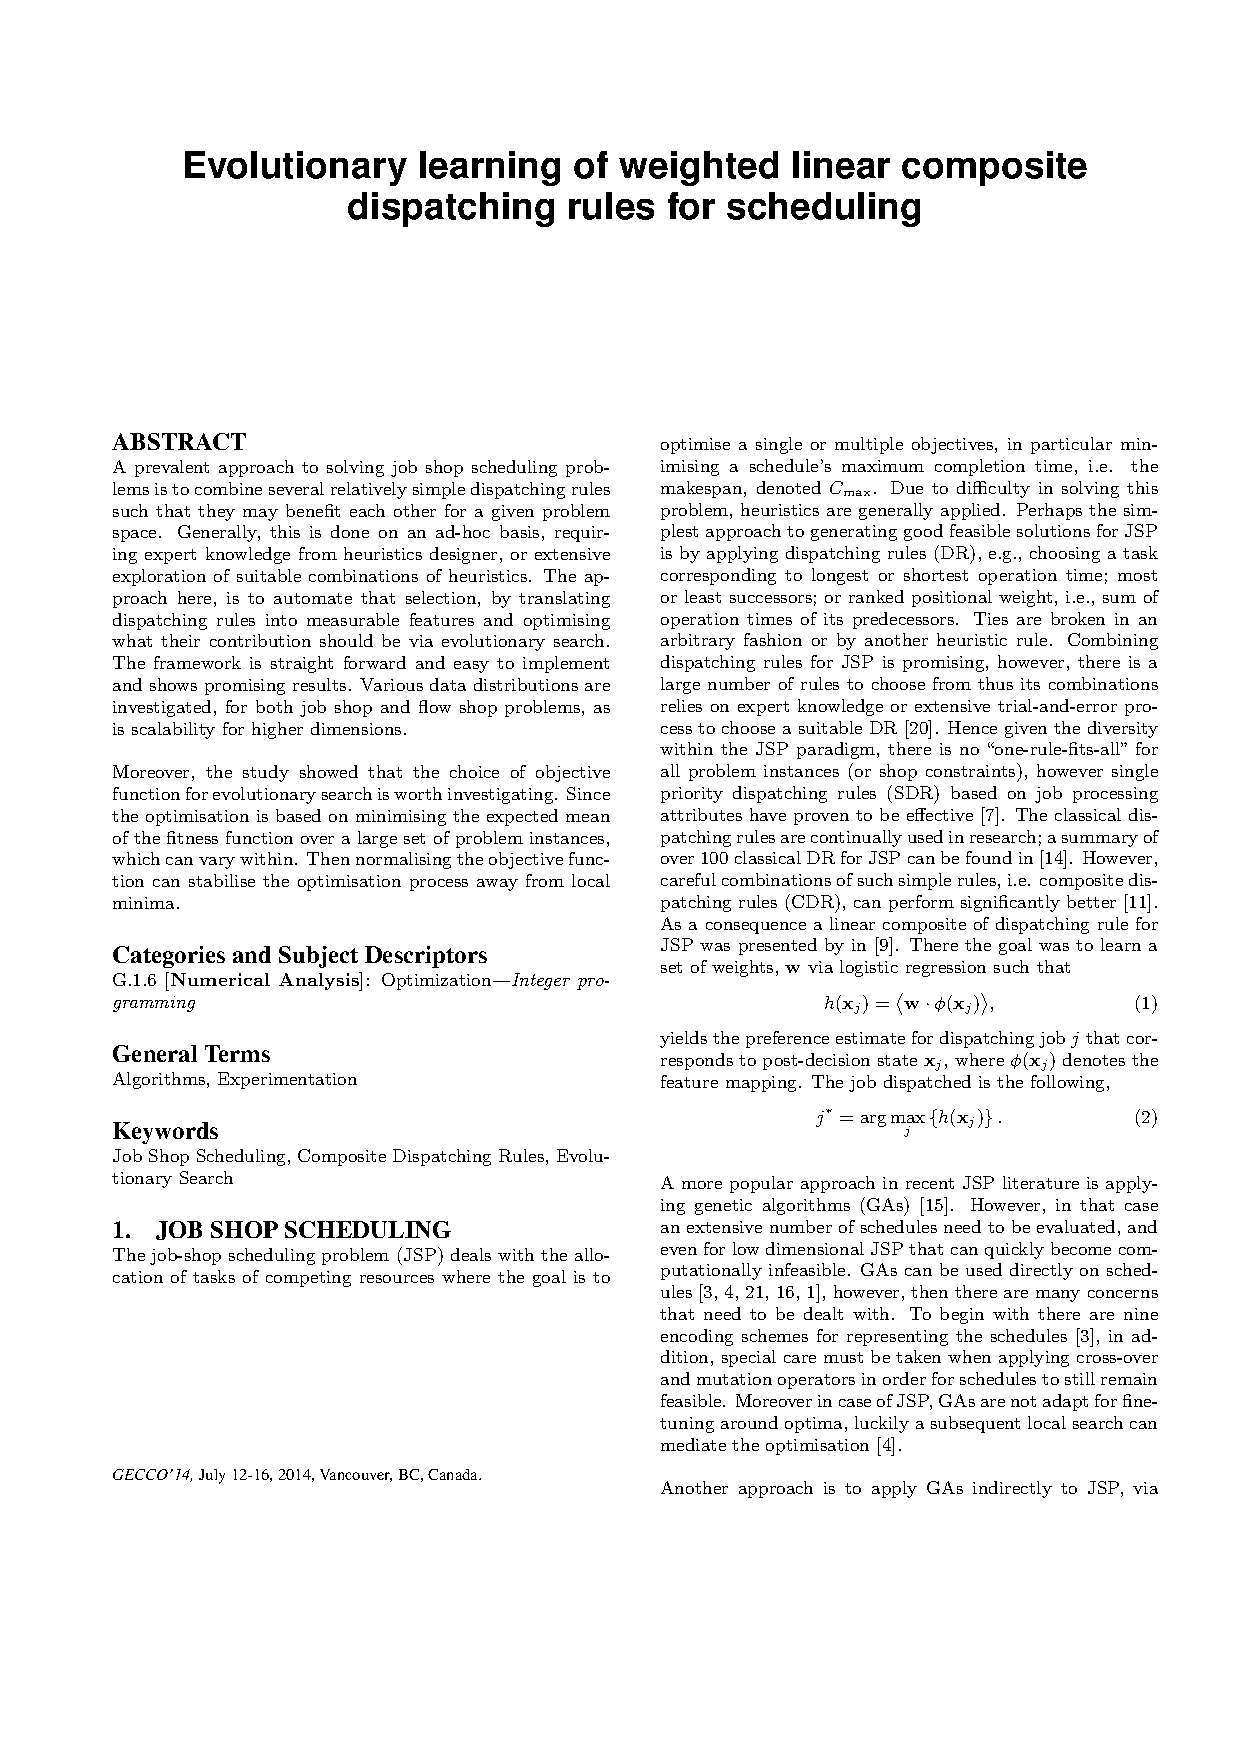
\includepdf[pages=1-7,pagecommand={\thispagestyle{fancy}},noautoscale,scale=0.8]{papers/gecco14_draft.pdf}

\section[AAAI14]{Generating Training Data for Learning Linear Composite Dispatching Rules for Scheduling}\label{app:aaai14}
Generating Training Data for Learning Linear Composite Dispatching Rules for Scheduling was submitted by \citeauthor{InRu14b} to twenty-sixth {Association for the Advancement of Artificial Intelligence} conference on \emph{Innovative Applications of Artificial Intelligence} (AAAI 26), July 29-31, 2014, Québec City, Canada. %The paper was been accepted as long paper (original novel and unpublished work) for presentation at the conference and inclusion in the proceedings. 

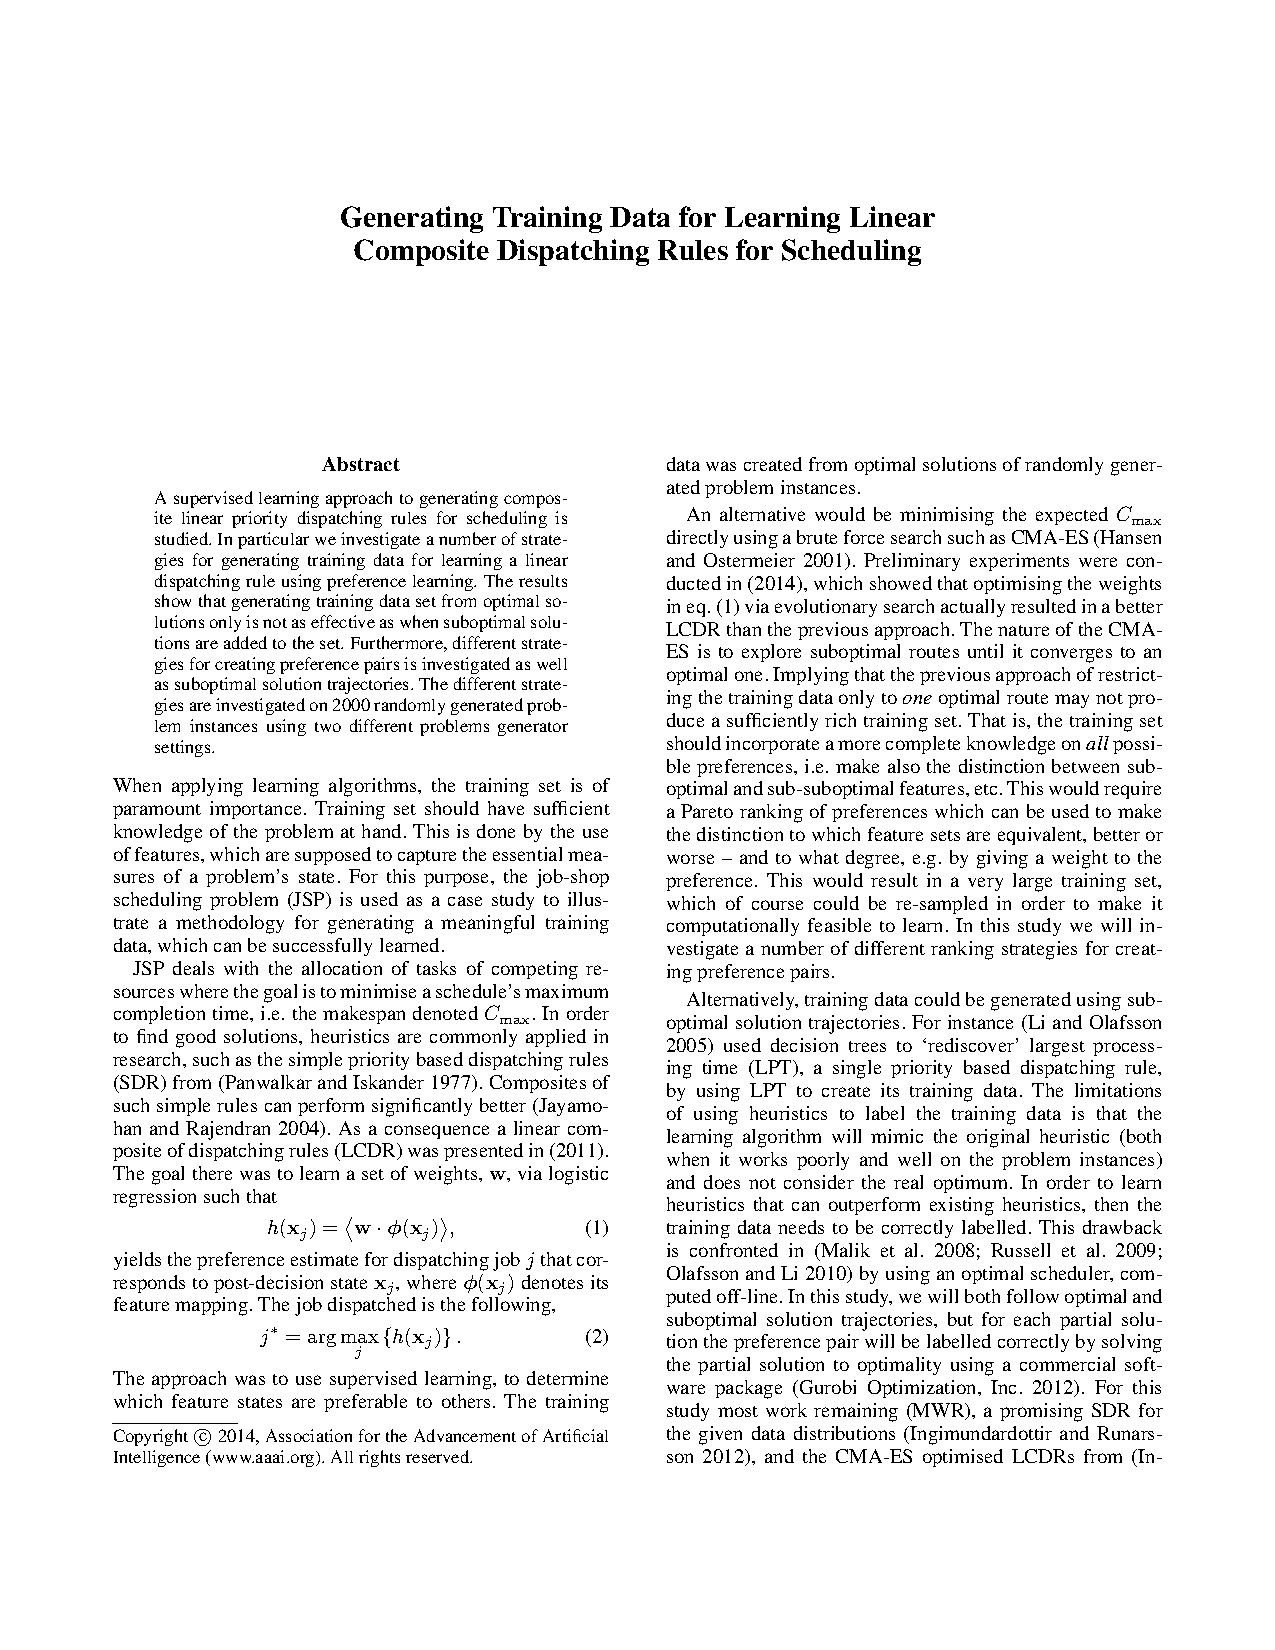
\includepdf[pages=1-7,pagecommand={\thispagestyle{fancy}}]{papers/aaai14_draft.pdf}
